%% 
%% Copyright 2007-2020 Elsevier Ltd
%% 
%% This file is part of the 'Elsarticle Bundle'.
%% ---------------------------------------------
%% 
%% It may be distributed under the conditions of the LaTeX Project Public
%% License, either version 1.2 of this license or (at your option) any
%% later version.  The latest version of this license is in
%%    http://www.latex-project.org/lppl.txt
%% and version 1.2 or later is part of all distributions of LaTeX
%% version 1999/12/01 or later.
%% 
%% The list of all files belonging to the 'Elsarticle Bundle' is
%% given in the file `manifest.txt'.
%% 

%% Template article for Elsevier's document class `elsarticle'
%% with numbered style bibliographic references
%% SP 2008/03/01
%%
%% 
%%
%% $Id: elsarticle-template-num.tex 190 2020-11-23 11:12:32Z rishi $
%%
%%
\documentclass[preprint,12pt]{elsarticle}

%% Use the option review to obtain double line spacing
%% \documentclass[authoryear,preprint,review,12pt]{elsarticle}

%% Use the options 1p,twocolumn; 3p; 3p,twocolumn; 5p; or 5p,twocolumn
%% for a journal layout:
%% \documentclass[final,1p,times]{elsarticle}
%% \documentclass[final,1p,times,twocolumn]{elsarticle}
%% \documentclass[final,3p,times]{elsarticle}
%% \documentclass[final,3p,times,twocolumn]{elsarticle}
%% \documentclass[final,5p,times]{elsarticle}
%% \documentclass[final,5p,times,twocolumn]{elsarticle}

%% For including figures, graphicx.sty has been loaded in
%% elsarticle.cls. If you prefer to use the old commands
%% please give \usepackage{epsfig}

%% The amssymb package provides various useful mathematical symbols
\usepackage{amssymb}
%% The amsthm package provides extended theorem environments
%% \usepackage{amsthm}

%% The lineno packages adds line numbers. Start line numbering with
%% \begin{linenumbers}, end it with \end{linenumbers}. Or switch it on
%% for the whole article with \linenumbers.
%% \usepackage{lineno}



\usepackage[labelfont=bf]{caption}
\usepackage[superscript,nomove]{cite}
\usepackage{csquotes}
\usepackage{wrapfig}
\usepackage[ruled,vlined,linesnumbered]{algorithm2e}
\usepackage{enumitem}
\usepackage{multirow}
\usepackage{caption}
\usepackage{subcaption}
\usepackage{todonotes}


\journal{Journal of Biomedical Informatics}

\begin{document}

\begin{frontmatter}

%% Title, authors and addresses

%% use the tnoteref command within \title for footnotes;
%% use the tnotetext command for theassociated footnote;
%% use the fnref command within \author or \address for footnotes;
%% use the fntext command for theassociated footnote;
%% use the corref command within \author for corresponding author footnotes;
%% use the cortext command for theassociated footnote;
%% use the ead command for the email address,
%% and the form \ead[url] for the home page:
%% \title{Title\tnoteref{label1}}
%% \tnotetext[label1]{}
%% \author{Name\corref{cor1}\fnref{label2}}
%% \ead{email address}
%% \ead[url]{home page}
%% \fntext[label2]{}
%% \cortext[cor1]{}
%% \affiliation{organization={},
%%             addressline={},
%%             city={},
%%             postcode={},
%%             state={},
%%             country={}}
%% \fntext[label3]{}

\title{Semantic Search for Large Scale Clinical Ontologies}

%% use optional labels to link authors explicitly to addresses:
%% \author[label1,label2]{}
%% \affiliation[label1]{organization={},
%%             addressline={},
%%             city={},
%%             postcode={},
%%             state={},
%%             country={}}
%%
%% \affiliation[label2]{organization={},
%%             addressline={},
%%             city={},
%%             postcode={},
%%             state={},
%%             country={}}

\author{Duy-Hoa Ngo}
\author{Simon Thomas}
\author{Bevan Koopman}
\affiliation{organization={CSIRO},%Department and Organization
            addressline={296 Herston Road}, 
            city={Brisbane},
            postcode={4029}, 
            state={Queensland},
            country={Australia}}



\begin{abstract}
%% Text of abstract

\end{abstract}

%%Graphical abstract
\begin{graphicalabstract}
%\includegraphics{grabs}
\end{graphicalabstract}

%%Research highlights
\begin{highlights}
\item Research highlight 1
\item Research highlight 2
\end{highlights}

\begin{keyword}
%% keywords here, in the form: keyword \sep keyword

%% PACS codes here, in the form: \PACS code \sep code

%% MSC codes here, in the form: \MSC code \sep code
%% or \MSC[2008] code \sep code (2000 is the default)

\end{keyword}

\end{frontmatter}

%% \linenumbers

%% main text






\section*{Introduction}
\label{sec:Introduction}

% An introduction of clinical terminology and Snomed CT
Data standardisation is an important and challenging goal in the field of medicine \cite{Benson2016}. One of the key elements required to achieve semantic interoperability between clinical systems is the availability of common ontologies that define the concepts in the domain. Currently, the most comprehensive clinical ontology available is SNOMED~CT, which contains more than 340,000 concepts and has been widely adopted in Electronic Health Record (EHR) systems worldwide. However, despite the availability and coverage of large ontologies such as SNOMED~CT, there are still many challenges with adoption and implementation. These revolve around two main issues: 1) much of the source data is free text and needs to be mapped to a standard ontology; 2) existing systems use their own code systems and it is not feasible to replace them with SNOMED~CT. 

The first problem can be addressed by using natural language processing (NLP), whereby free text is analysed to identify relevant concepts. This process is called \textit{information extraction} \cite{Jurafsky2009} and it has been studied extensively in the biomedical domain. The process is typically divided in two phases: identifying the spans of text that represent relevant concepts and mapping these spans to concepts in a chosen ontology (also referred to as \textit{concept normalisation}).

% Use cases explained in more detail
The second problem can be addressed by mapping between ontologies. For any ontology of considerable size these maps cannot be generated manually and require at least partial automation. This area of research is called \textit{ontology matching}\cite{Euzenat2013}. Some of the most important elements that inform the matching process are the labels, synonyms and descriptions of the concepts.

% What we built and intro to use cases
Tailored solutions exists for both the concept normalisation problem and the ontology matching problem. However, these tend to be very specific to the particular use case. Instead, in this paper we propose a generalised method for searching large ontologies such as SNOMED~CT, using short spans of text as input. This method can be used generically for both concept normalisation and ontology matching. A novel algorithm is presented, based on deep-learning-derived word representations, that is capable of finding good candidate concepts, even in the absence of common vocabulary. Input to the algorithm can be free text, when doing concept normalisation, or a concept from a source ontology, when doing ontology matching. 

We empirically evaluate our method in a number settings --- both concept normalisation and ontology matching. The results show that our method can effectively find relevant concepts, outperforming a number of comparison baselines. In addition, we show that our method is particularly suited to finding concepts where the input shares little or no common terms with the relevant concept. 

\section*{Related Work}
\label{sec:RelatedWorks}
% Talk about ontology searching

The problem of searching large ontologies has been studied in the context of data entry. Sevenster et al. \cite{sevenster2012} proposed and evaluated an autocompletion algorithm for large medical ontologies and showed that a multi-prefix matching approached performs better than the baseline approach that only completes the entered string to the right. A modified version of this algorithm is implemented in Ontoserver \cite{metke2018}, a high-performance FHIR terminology server, and it is used by default to do value set expansions\footnote{In FHIR, this is the operation used to implement auto-complete style widgets for data capture.}. However, this algorithm doesn't perform well on other tasks where the input strings are not partial prefixes but rather full words or short sentences. Also, the algorithm uses standard string matching so it only works well when the queries use the same vocabulary as the ontology being searched.

% Talk about related work in the concept normalisation use case
Searching ontologies has also been studied in the area of information extraction, specifically in the concept normalisation step where a span of text that has been identified as being relevant is mapped to a concept in an ontology. Wang et. al. \cite{wang2018} wrote an extensive literature review on clinical information extraction. An example of a state of the art algorithm specifically designed for the concept normalisation step can be found in the work of Luo et al. \cite{luo2019}. % expand the description a bit

Finally, although not specific to ontology search, there is also relevant related work in the area of information retrieval (IR). Recently, advanced neural network methods have been developed to learn semantic representations of words and overcome the vocabulary mismatch problem of traditional IR models. Popular models that follow this trend include \textit{Word2Vec} \cite{Mikolov2013}, \textit{GloVe} \cite{Jeffrey2014} and \textit{fastText} \cite{Piotr2016}. Their underlying idea is based on the distributional hypothesis in linguistics, i.e., words that are used and occur in the same contexts tend to purport similar meanings\footnote{https://en.wikipedia.org/wiki/Distributional\_semantics}. Those neural networks are trained with large data resources by unsupervised learning algorithms. Once the training is finalised, every word located in the model's dictionary will be encoded by a fixed length embedding vector. Then, those embedding vectors can be used as inputs to a combination function (e.g., average function) or another neural network model to derive an embedding vector of a query or a document. A limitation of these methods is that once the training is completed, the embedding vectors are static, which means that an embedding vector of a given word is always the same regardless of the context of use. Therefore, they may face issues with polysemy when a word might have a different meaning in a specific context.

%A search engine is an information retrieval system that returns ranked relevant results (documents) to a user-submitted query according to their relevance scores. Its fundamental working principle is to encode the user queries and objects in a target database into some meaningful representation, thus the searching algorithms can efficiently score the relevance between a query representation and documents' representation. The \textbf{Vector Space Model} has been used as the main representation approach for natural language in modern search engine systems.  
% In these models, user text queries, as well as to-be-searched documents, are transformed into numeric vectors in a high-dimensional vector space. Their relevance score can be computed using vector similarity (distance) metrics such as Euclidean distance, Manhattan distance or Cosine similarity. 

%Generally, \textbf{TF-IDF} (term frequency–inverse document frequency) is a basic and popular approach for representing embedding vectors for text data. It treats each document and query as a vector of keywords in which the keywords' weights represent their importance  in document and query within the entire document collection. BM25 \cite{Stephen2009} is one of the most popular ranking functions used by search engines on top of a \textbf{TF-IDF} vector space to estimate the relevance of documents to a given search query. A strength of the this approach is that it performs best when users select the {right} keywords that match the contents. However, a limitation of this approach is that it makes no use of semantic similarities between words, which may return poor results when the query keywords are not selected properly. That is one of the major gaps addressed by semantic search. A semantic search engine differs from the traditional term-based search in that it attempts to represent a user's query and documents in a semantic vector space model, where the closer the objects are located in the space, the higher semantic similarity scores they have. In this way, the model is not dependent on the individual terms used to describe something and instead relies on its meaning (e.g., `heart attack' and `myocardial infarction' will have high semantic similar even though they have no term overlap).

%To overcome the word mismatch problem of the \textbf{TF-IDF} based traditional search engines, advanced neural network method have been widely adopted to learn semantic representation of words. Popular models in this trend are \textbf{Word2Vec} \cite{Mikolov2013}, \textbf{GloVe} \cite{Jeffrey2014} and \textbf{fastText} \cite{Piotr2016}. Their underlying idea is based on the distributional hypothesis in linguistics, i.e. words that are used and occur in the same contexts tend to purport similar meanings\footnote{https://en.wikipedia.org/wiki/Distributional\_semantics}. Those neural network are trained with large data resources by unsupervised learning algorithms. Once the training is finalised, every word located in the model's dictionary will be encoded by a fixed length embedding vector. Then, those embedding vectors can be used as inputs to a combination function (e.g., average function) or another neural network model to derive an embedding vector of a query or a document. A limitation of those methods is that once the training is completed, the embedding vectors are static, which means that an embedding vector of a given word is always the same regardless of the context of use. Therefore, they may face issues with polysemy when a word might have a different meaning in a specific context.

Several contextualised word embedding methods based on deep long short-term memory (LSTM) architectures, such as \textit{CoVe} \cite{Bryan2017}, \textit{ELMO} \cite{Matthew2018} and \textit{FLAIR} \cite{Akbik2018}, have been proposed to improve the understanding of words and sentences. The main difference with the static word embedding methods is that the words' embedding vectors are dynamically generated according to which context they have been used, i.e., surrounding words in a given sequence. Recently, \textit{transformer}-based approaches like \textit{BERT} \cite{Devlin2019}, \textit{XLNet} \cite{Zhilin2019}, \textit{RoBERTa} \cite{Yinhan2019} have been proposed and achieved  state-of-the-art results over most NLP downstream tasks. A key idea in these methods is that the meaning of a word in a sequence is represented by how much attention of that word attracts the other words in the sequence. Once the training of those models completes, they output a list of embedding vectors for all tokenised words of a given sequence. Then, those embedding vectors can be combined in different strategies to derive a semantic embedding vector for an input sequence.

A special feature of a search engine designed to search large ontologies is that the to-be-searched documents are concept labels, which are usually short and, therefore, sentence embedding methods are highly relevant because they can be used to compute semantic relatedness between this type of label. Recently, many sentence embedding methods, for example \textit{Doc2Vec} \cite{Quoc2014},  \textit{Skip-Thought} \cite{Ryan2015}, \textit{InferSent} \cite{Conneau2017}, \textit{Universal Sentence Encoder} \cite{Daniel2018} and the \textit{Sentence-BERT} model \cite{Reimers2019} have been proposed and have achieved good results in various natural language understanding tasks such as sentiment analysis, text classification, question answering and semantic textual similarity. \textit{Doc2Vec} is an extension of \textit{Word2Vec} that is trained with large, unlabelled text data. \textit{Skip-Thought} is another extension of the Skip gram \textit{Word2Vec} model that tries to predict the surrounding sentences of a given sentence. \textit{Universal Sentence Encoder} trains a transformer network which augments unsupervised learning whereas \textit{InferSent} trains a Siamese BiLSTM network with a max-pooling layer on top. Similar to the \textit{InferSent} architecture, \textit{Sentence-BERT} replaces a BiLSTM network with a BERT network and outperforms the other state-of-the-art methods on common semantic textual similarity and transfer learning tasks. These models have been trained on natural language inference data sets \cite{Samuel2015, Adina2018}, in which, an input to a learning model is a pair of sentences and the output is an inferred relation between them.

The algorithm we propose in this paper is most similar to \textit{Sentence-BERT} \cite{Reimers2019}. Sentence-BERT uses a Siamese architecture, and classification and regression objective functions. Our approach instead, uses a Triplet network \cite{Hoffer2015}, which processes three inputs in parallel, and a triplet loss function, which is a learning to rank metric for the three inputs.

\section*{Method}
\label{sec:Method}

In this section we provide the details of our semantic search engine model for large scale clinical ontologies. First, we give an overview of the model and its components, and explain how to rank results for a given query. Then, we outline our training procedure, optimization objective in developing the model.

% \subsection*{Intuition}
% \label{sec:Intuition}

The main idea of this model is to transform every concept's label into appropriate embedding vectors in a vector space so their locations preserve the semantic relations between concepts in the ontology. Figure~\ref{fig:Fatigue} shows an example that illustrates this idea. The example shows that the concept \texttt{Asthenia} has three synonyms: {\textit{Weakness - general}}, {\textit{Lassitude}} and {\textit{Debility}}. Due to the characteristics of synonymy, we would expect that the distance between the embedding vectors of synonyms, e.g., {\textit{Asthenia}} vs. {\textit{Weakness - general}}, would be smaller than the distance between the vectors of labels of concepts that are not synonyms, e.g., {\textit{Asthenia}}vs. {\textit{Fatigue}} or {\textit{Exhaustion}}.

\begin{figure}[htbp]
	\centering
		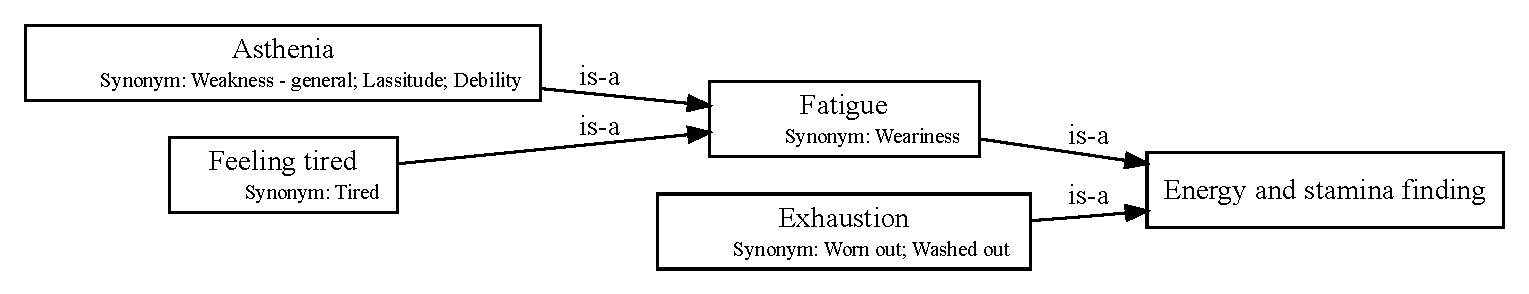
\includegraphics[width=0.9\textwidth]{figures/Asthenia.eps}
	\vspace{-0.5em}
	\caption{A SNOMED CT fragment for Asthenia, Feeling tired, Fatigue, Exhaustion and Energy and stamina finding.}
	\label{fig:Fatigue}
\end{figure}

 
On the other hand, the concept \texttt{Feeling tired} is a sibling of the concept \texttt{Asthenia} because they both are children of the concept \texttt{Fatigue}. By applying the distance calculation method on the tree structure, the distance between two concepts is computed by the sum of the distances from those concepts to their lowest common ancestor. Therefore, we would also expect the  distance between embedding vectors of a concept's label to its direct parent concept's label to be smaller than the distance of that concept's label to its sibling concept's label. In this example, the distance between concept \texttt{Asthenia} and concept \texttt{Fatigue} must be smaller than the distance between concept \texttt{Asthenia} and its sibling \texttt{Feeling tired}. Again, because {\textit{Lassitude}} is a synonym label of \texttt{Asthenia} and {\textit{Weariness}} is a synonym label of \texttt{Fatigue}, we would infer that a embedding vector of {\textit{Lassitude}} is located closer to a embedding vector of {\textit{Weariness}} than to a embedding vector of  {\textit{Feeling tired}}. The intuition of distance comparison based on synonymy and tree-based distance can be applied to all concepts in an ontology.

\subsection*{Label embedding with Triplet-BERT model}
\label{sec:TripletBERT}

In order to achieve a vector space model that observes the properties described in the previous section, a Triplet-Bert model was trained to produce a semantic embedding vector for short text spans such as concepts' labels or user queries. The Triplet-Bert model is a kind of Triplet network \cite{Hoffer2015} and it was mentioned by Reimers et al \cite{Reimers2019}. It consists of three instances of the same \textbf{embedding layer} containing a shared BERT network and a pooling layer (see Figure \ref{fig:Triplet}). It requires three text inputs, which are fed into the network at the same time, and represent three different roles: an \textbf{anchor} input, a \textbf{positive} input and a \textbf{negative} input. In this work, an \textbf{anchor} input is a user query (e.g., {\textit{Weakness - general}}); a \textbf{positive} input is a label of a high relevant concept (e.g., {\textit{Asthenia}}) to the user's query; and a \textbf{negative} input is a label of a less relevant concept (e.g., {\textit{Exhaustion}}) to the query. 

\begin{figure}[htbp]
	\centering
		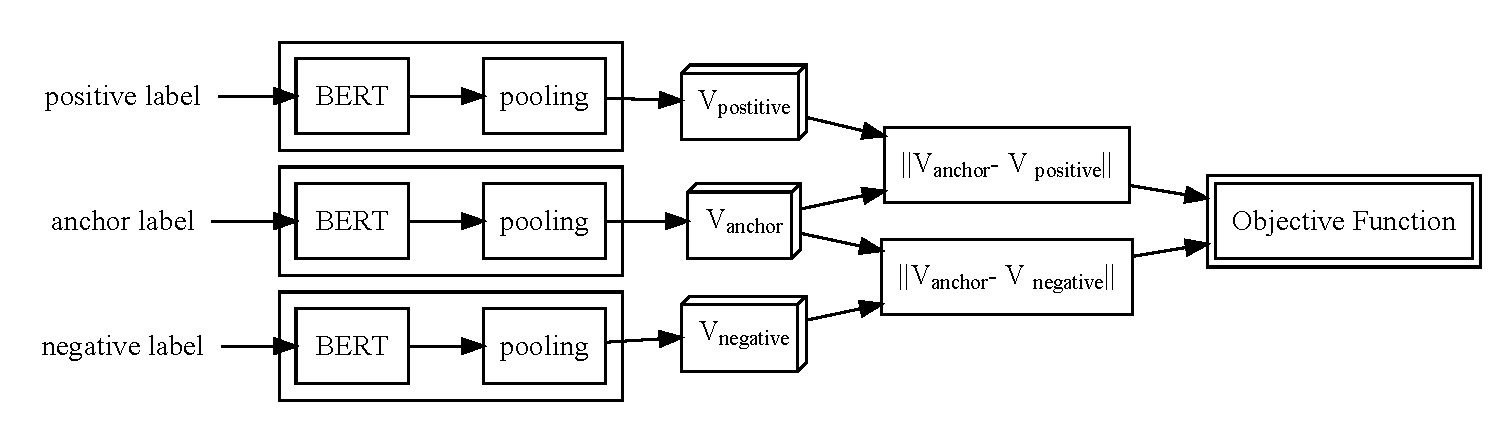
\includegraphics[width=0.8\textwidth]{figures/Triplet2.eps}
	\vspace{-0.5em}
	\caption{Triplet-BERT model architecture}
	\label{fig:Triplet}
\end{figure}

The objective of a Triplet-BERT model is to train its parameters so at the end, the encoded embedding vector of the \textbf{anchor} input is closer to the embedding vector of the \textbf{positive} input than that to the embedding of the \textbf{negative} input. Firstly, each input is fed into a BERT network to produce a list of intermediate embedding vectors, then, a pooling layer combines these vectors to produce a summary embedding vector for a given input. Now, after receiving three embedding vectors $V_{anchor}$, $V_{positive}$ and $V_{negative}$ for \textbf{anchor}, \textbf{positive} and \textbf{negative} inputs respectively, the model computes distances between the embedding vector of the anchor input against the embedding vectors of positive and negative inputs. Finally, the Objective Function module compares the two distances and indicates whether the model needs to adjust its parameters through the back propagation algorithm.  
Once the training has completed, the \textbf{embedding layer} is used to produce embedding vectors for any user text query as well as concept labels in the ontology. In order to rank results for a given query, the cosine similarity metric is used to compute relevance scores between the user queries and the concepts' labels. 
 

\subsection*{Training Data Set}
\label{sec:TrainingDatasets}
Deep neural network methods had been recently used to develop sentence embedding models. Due to the huge number of parameters in deep neural networks, these models require a significant amount of training data. Some common published data sets used for training sentence embedding are the Stanford Natural Language Inference (SLNI) data set \cite{Samuel2015}, the Multi-Genre NLI data set (MLNI) \cite{Adina2018} and the Semantic Textual Similarity (STS) data set \cite{Daniel2017}. Each entry in those data sets consists of a pair of sentences and a label that is either a relationship type or a semantic similarity score. These entries cannot be used in our Triplet network because it requires three input sentences at the same time. Therefore, we propose a method to generate a data set for training our Triplet network (see Algorithm \ref{Alg:dataset}) based on the aforementioned intuition about distances of concepts in an ontology's hierarchy. The whole data set was generated from SNOMED~CT and the Human Phenotype Ontology (HPO). Each entry in the data set consists of three strings following the same order: an \textbf{anchor} label, a \textbf{positive} label and a \textbf{negative} label.  In total, the generated data set contains nearly \textbf{4 millions} entries, which are then split into \textit{training}, \textit{development} and \textit{testing} data sets with ratio of $90\%$, $5\%$ and $5\%$ respectively.

\begin{algorithm}[htbp]
\SetAlgoLined
\KwIn{T: Ontology}
\KwOut{$D_{train}$, $D_{dev}$, $D_{test}$}
D $\gets$ $\emptyset$\\
\ForEach{concept $\in$ T}{
    $conceptLabels$ $\gets$ getLabels($concept$, T) \\
    $directParents$ $\gets$ getParents($concept$, T)\\
    $otherConcepts$ $\gets$ getSiblings($concept$, T) $\cup$ getSiblings($directParents$, T)\\
    \ForEach{($label_{1}$ $\ne$ $label_{2}$) $\in$ conceptLabels}{
        $parentLabel$ $\gets$ getRandomLabel($directParents$, T)\\
        $otherLabel$ $\gets$ getRandomLabel($otherConcepts$, T)\\
        addToDataset(D, anchor=$label_{1}$, positive=$label_{2}$, negative=$parentLabel$)\\
        addToDataset(D, anchor=$label_{1}$, positive=$label_{2}$, negative=$otherLabel$)\\
        addToDataset(D, anchor=$label_{1}$, positive=$parentLabel$, negative=$otherLabel$)\\
    }
}
$D_{train}$, $D_{dev}$, $D_{test}$ $\gets$ splitTrainDevTest(D)
\caption{Generate training data from ontology for Triplet network}
\label{Alg:dataset}
\end{algorithm}

% As the names suggest, function \texttt{getLabels}  returns a list of concept's labels and synonyms; functions \texttt{getParents}, \texttt{getSiblings} and \texttt{getUncles} returns lists of parents, siblings and uncles of the concept located in the hierarchy of the terminology system; function \texttt{getRandomLabel} returns a random label (including synonymous label) of a concept randomly selected from a list of given concepts. 


\subsection*{Training Details}
\label{sec:TrainingDetails}

\textbf{BERT network}. Transfer learning was used to fine-tune BERT parameters. In this work, we adopted BioBert-Base v1.1 \cite{Lee2019} --- a state-of-the-art biomedical language representation model, which has been widely using biomedical natural language processing tasks. 

\textbf{Pooling layer}. The pooling layer is added on top of the BERT network to get an embedding vector for a given text input. Different strategies can be used to work with BERT's output embedding vectors, however, according to Reimers et al \cite{Reimers2019}, the \texttt{MEAN} strategy achieved a better result than the others. Therefore, we chose the \texttt{MEAN} strategy for the pooling layer to produce a fixed size, i.e., a 768-dimensional embedding vector for the given text input.

\textbf{Distance metric}. We use Euclidean distance to compute distances between the anchor embedding vectors ($V_{anchor}$), the positive embedding vectors ($V_{positive}$) and the negative embedding vectors ($V_{negative}$).

\textbf{Objective function}. The objective of our model is to move the anchor embedding vector ($V_{anchor}$) closer to the positive embedding vector ($V_{positive}$) and far away from the negative embedding vector ($V_{negative}$). Therefore, we minimize the following objective function to tune the model's parameters:
\[ loss = \max(||V_{anchor} - V_{positive}|| - ||V_{anchor} - V_{negative}|| + m, 0)\]
Here, a small margin value $m$ is used to push the distance $||V_{anchor} - V_{negative}||$ being at least $m$ higher than the distance $||V_{anchor} - V_{positive}||$. Otherwise, the $loss\_value$ is positive, thus its derivatives to model' parameters are not 0, so the back propagation algorithm will update the model's parameters. In the training phase, we fix $m = 0.1$.

\textbf{Training settings}. Our model was trained in 5 epochs. We set a batch-size of 32, Adam optimizer with learning rate 2e-5, and a linear learning rate warm-up over 10\% of the training data. The training process was done in 40 hours with one GPU with 32G RAM, using Python 3.6, Pytorch 1.6 and CUDA 10.1. The Triplet-BERT codes was derived from Sentence-BERT \cite{Reimers2019} codes by replacing siamese network by triplet network.

\section*{Evaluation}
\label{sec:Evaluation}

In this section, we firstly describe how to evaluate the performance of our semantic search system and related evaluation metrics. Next, we present data sets used in the evaluation and finally we analyze the experimental results.

As our evaluation measure we use Hits@K. For a given query, Hits@K is 1 if the relevant concept is found in the top $K$ results; otherwise it is 0. In our evaluation, we used Hits@1, Hits@5 and Hits@10. Additionally, in order to measure the usefulness of the list of returned results for a given query, Normalized Discounted Cumulative Gain (nDCG) and Mean Reciprocal Rank (MRR) were used. Their underlying assumption is that the higher the relevant results are ranked, the more gain the user receives. Therefore, the \textit{ideal ranking} would first return the result with the highest relevance level, then the next highest relevance level, etc. nDCG@K measures the performance of a search system based on the relevance order of the $K$ returned results against the ideal ranking order. In our evaluation, we used nDCG@1, nDCG@5 and nDCG@10.

\subsection*{Data Sets for Evaluation}
\label{sec:DatasetEvaluation}

\section*{Conclusion}












%% The Appendices part is started with the command \appendix;
%% appendix sections are then done as normal sections
%% \appendix

%% \section{}
%% \label{}

%% If you have bibdatabase file and want bibtex to generate the
%% bibitems, please use
%%
%%  \bibliographystyle{elsarticle-num} 
%%  \bibliography{<your bibdatabase>}

%% else use the following coding to input the bibitems directly in the
%% TeX file.

\begin{thebibliography}{00}

%% \bibitem{label}
%% Text of bibliographic item

\bibitem{}

\end{thebibliography}
\end{document}
\endinput
%%
%% End of file `elsarticle-template-num.tex'.
